\chapter{Research Methodology}

\section{Choice of technology}
Even though most tools for the semantic web are written in Java, some open source libraries for Python have become availabe in recent years \cite{w3java}. Python then became an easy choice for handling JSON files and creating RDF triples. For handling the automatic workflow scheduling, we opted for Apache Airflow as we had learned about this in class.


\section{Data collection process}
Statens vegvesen \cite{statensvegvesen} provides an API for their parking data in JSON format. As the API only gives access to subsets of the data, we have created a program that fetches the complete dataset and creates a single JSON file.

This data is fed to a program that combines our ontology and the parking data, creates RDF triples in a XML/RDF file format. The program uses data from the norwegian postal and logistics company Bring \cite{bring} to match postal codes from Statens vegvesen's data with municipalities codes. These codes are then linked with Wikidata \cite{wikidata}.


\section{System architecture}

\begin{figure}[H]
	\centering
	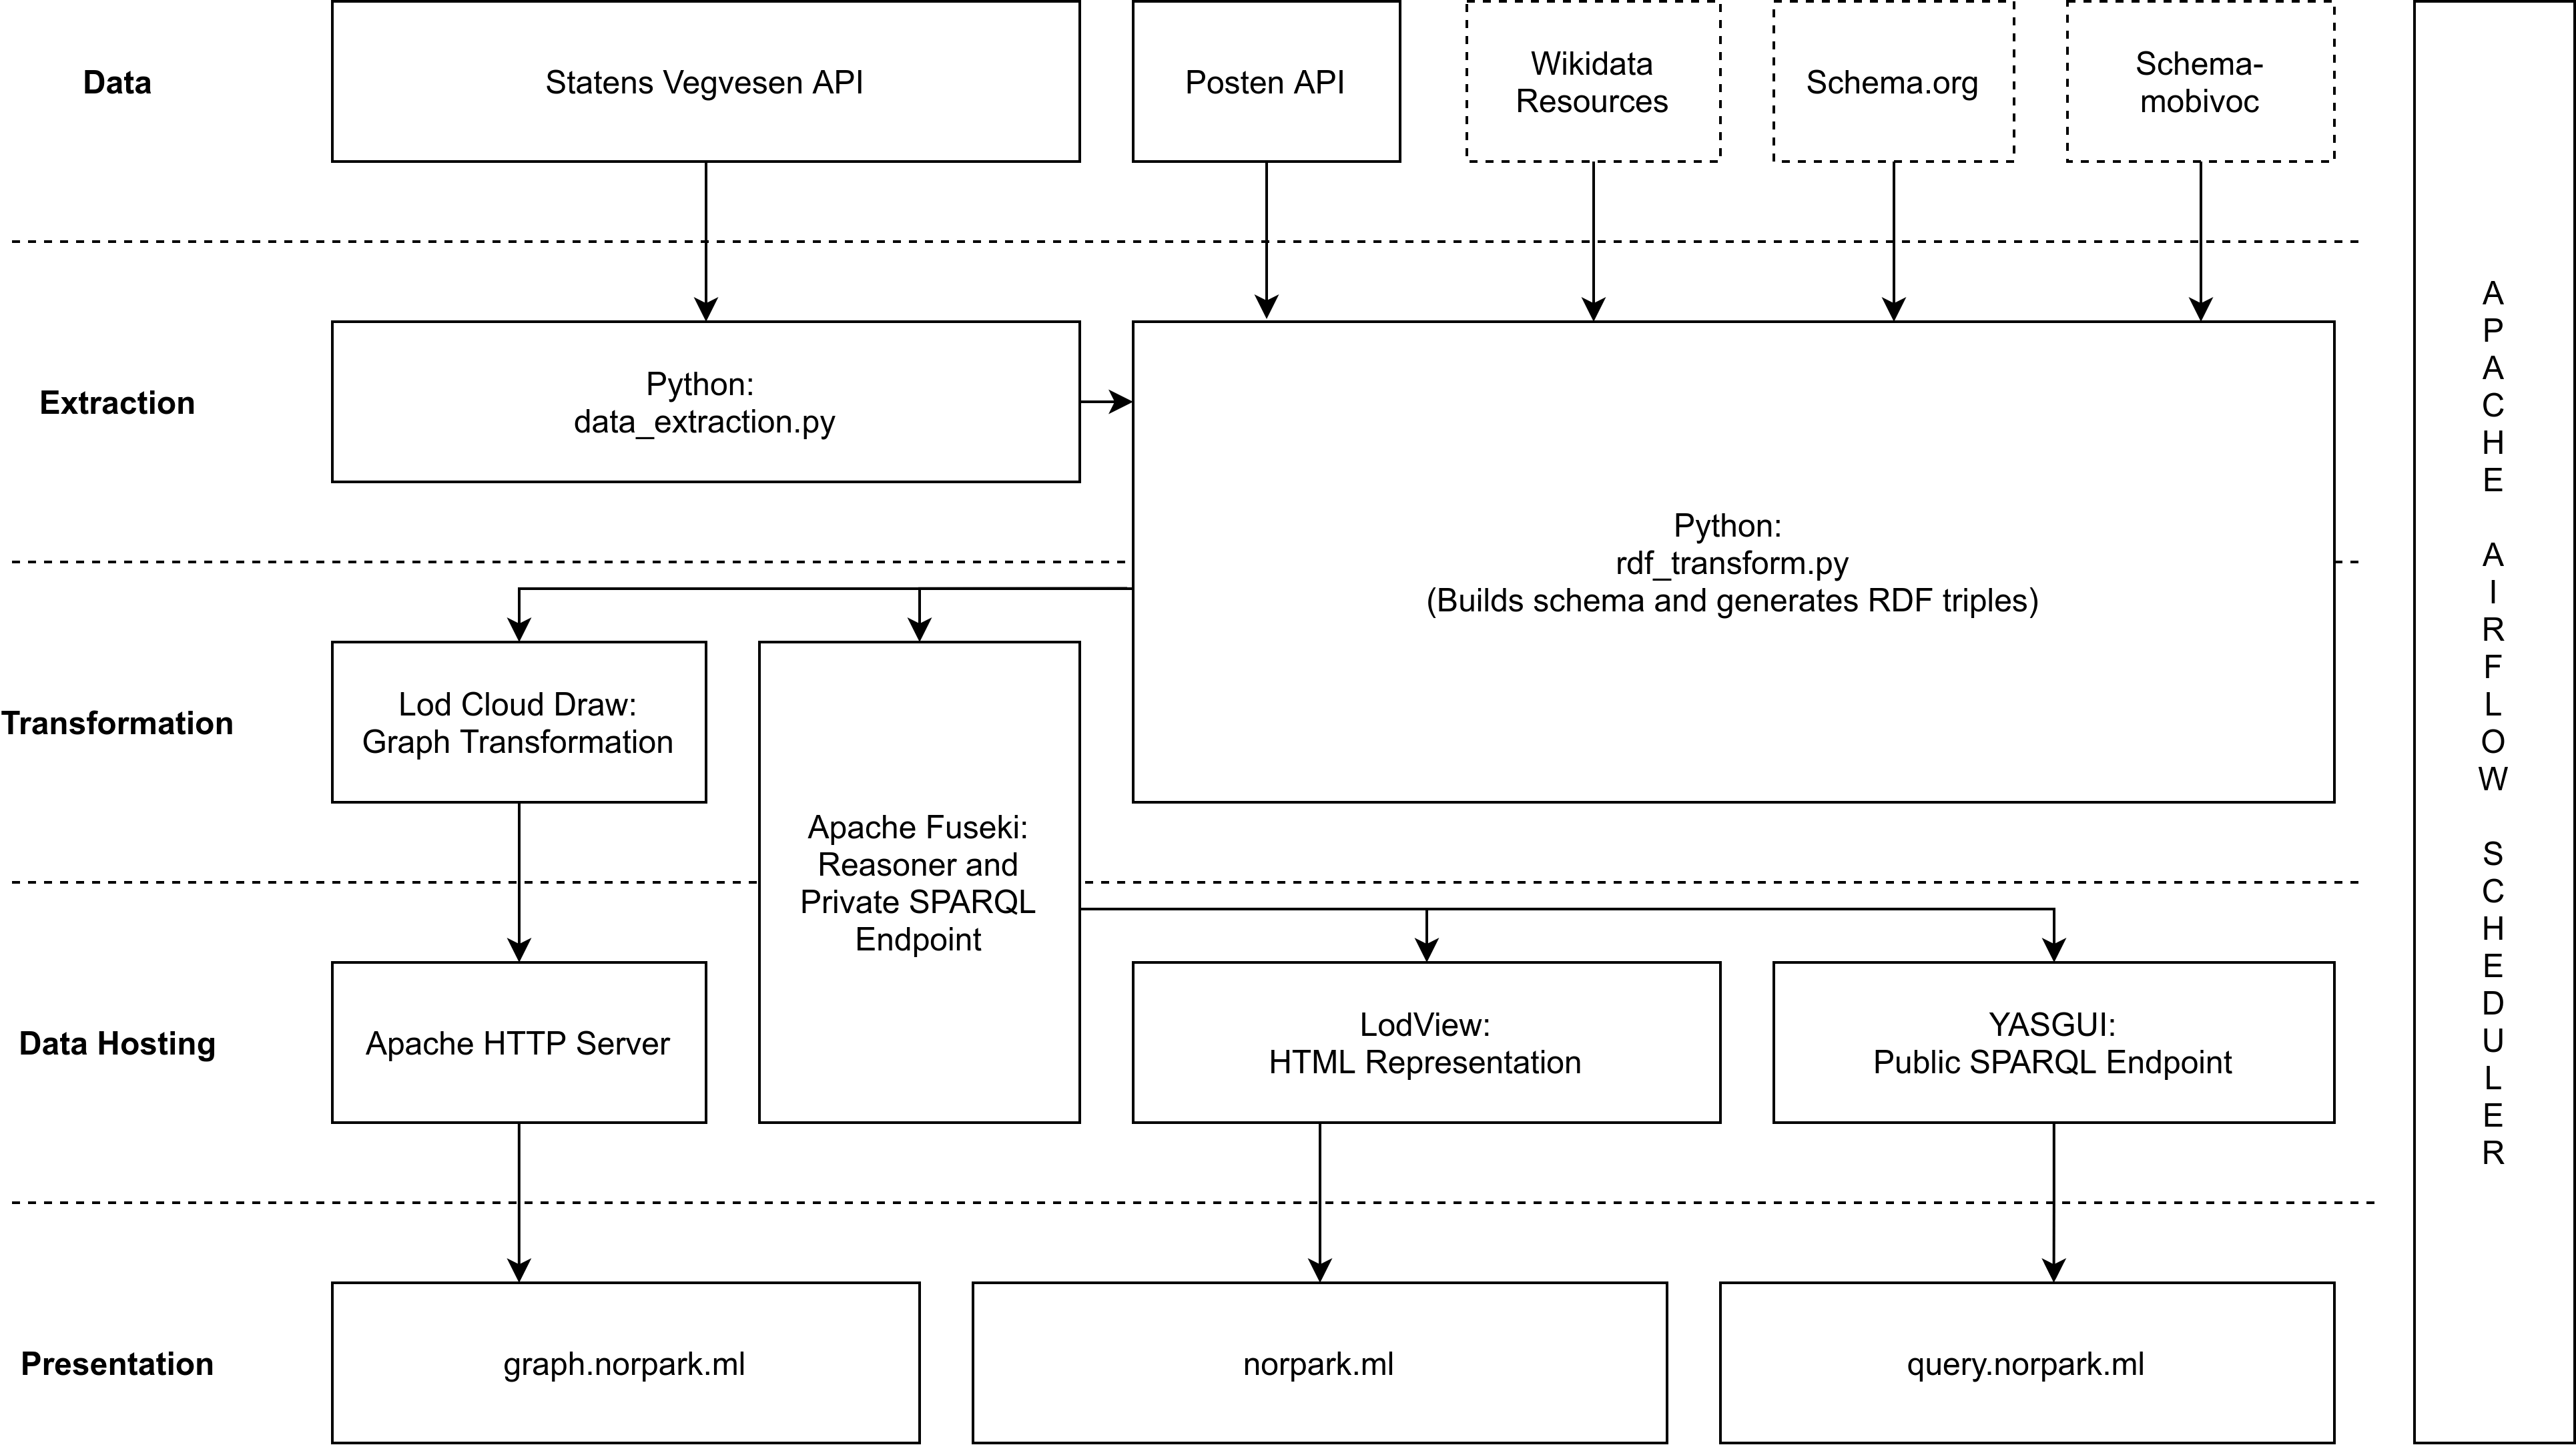
\includegraphics[width=\linewidth]{figures/system-architecture.png}
	\caption{The system architecture}
\end{figure}



